\documentclass[a4paper,crop=false]{standalone}
% \usepackage{amsmath}
% \usepackage{amssymb}
% \usepackage{fullpage}
% \usepackage[compat=1.1.0]{tikz-feynman}
% \usepackage{wrapfig}
% \usepackage{hyperref}
% \usepackage{graphicx,subcaption,caption}
\begin{document}
We can also have some intervalley potential which connects both the valley with an interaction strength $V_2$
        \begin{equation}
            H_{intval} = \frac{V_2}{2!2!} \Psi^{\dagger}_{1,k_4}\Psi^{\dagger}_{2,k_3}\Psi_{2,k_2}\Psi_{1,k_1} + \frac{V_2}{2!2!} \Psi^{\dagger}_{2,k_4}\Psi^{\dagger}_{1,k_3}\Psi_{1,k_2}\Psi_{2,k_1}
        \end{equation}

        This kind of interaction allows the vertex of the type shown in the figure \ref{fig:vertex2}. This allowed the one loop diagrams of the type shown in \ref{fig:oneloopv2}
        \begin{figure*}[h]
            \documentclass{standalone}
% \usepackage[compat=1.1.0]{tikz-feynman}

\begin{document}
    \begin{subfigure}[t]{0.3\textwidth}
            \begin{tikzpicture}
                \begin{feynman}
                    \vertex (a)[dot,label=left:\(V_2\)];
                    \vertex [above left=of a] (f1) {\(1,k_4\)};
                    \vertex [above right=of a] (f2) {\(2,k_3\)};
                    \vertex [below left=of a] (i1) {\(1,k_1\)};
                    \vertex [below right=of a] (i2) {\(2,k_2\)};
                    \diagram*{
                        (i1)--[fermion](a)--[fermion](f1),
                        (i2)--[fermion](a)--[fermion](f2);
                    };
                \end{feynman}
            \end{tikzpicture}
            \caption{$V_2$ vertex}
            \label{fig:vertex2}
        \end{subfigure}
        \begin{subfigure}[t]{0.3\textwidth}
            \begin{tikzpicture}
                \feynmandiagram [horizontal=b to c, layered layout] {
                a -- [fermion,edge label'=\(2\)] b [label=below:\(V_2\)] -- [fermion, out=135, in=45, loop, min distance=3cm,edge label'=\(1\)] b -- [fermion,,edge label'=\(2\)]c,
                };
            \end{tikzpicture}
            \caption{tadpole}
            \label{fig:tadpolefromV2}
        \end{subfigure}
        \begin{subfigure}[t]{0.4\textwidth}
            \begin{tikzpicture}
                \begin{feynman}
                    \vertex (a)[dot,label=below:\(V_2\)];
                    \vertex [right=of a] (b)[dot,label=below:\(V_2\)];
                    \vertex [below left=of a] (i1) {\(1\)};
                    \vertex [below right=of b] (i2) {\(1\)};
                    \vertex [above left=of a] (f1) {\(1\)};
                    \vertex [above right=of b] (f2) {\(1\)};
                    \diagram*{
                        (i1)--[fermion](a)--[fermion](f1),
                        (i2)--[fermion](b)--[fermion](f2);
                        (a)--[fermion,out=45,in=135,edge label=\(2\)](b);
                        (b)--[fermion,out=-135,in=-45,edge label=\(2\)](a);
                    };
                \end{feynman}
            \end{tikzpicture}
            \caption{ZS for $V_1$}
            \label{fig:oneloop2}
        \end{subfigure}
        \begin{subfigure}[t]{0.3\textwidth}
            \begin{tikzpicture}
                \begin{feynman}
                    \vertex (a)[dot,label=below:\(V_2\)];
                    \vertex [right=of a] (b)[dot,label=below:\(V_2\)];
                    \vertex [below left=of a] (i1) {\(1\)};
                    \vertex [below right=of b] (i2) {\(2\)};
                    \vertex [above left=of a] (f1) {\(2\)};
                    \vertex [above right=of b] (f2) {\(1\)};
                    \diagram*{
                        (i1)--[fermion](a)--[fermion](f1),
                        (i2)--[fermion](b)--[fermion](f2);
                        (a)--[fermion,out=45,in=135,edge label=\(1\)](b);
                        (b)--[fermion,out=-135,in=-45,edge label=\(2\)](a);
                    };
                \end{feynman}
            \end{tikzpicture}
            \caption{$ZS'$ for $V_2$}
            \label{fig:oneloop3}
        \end{subfigure}
        \begin{subfigure}[t]{0.3\textwidth}
            \centering
            \begin{tikzpicture}
                \begin{feynman}
                    \vertex (a)[dot,label=below:\(V_2\)];
                    \vertex [above=of a] (b)[dot,label=below:\(V_2\)];
                    \vertex [below left=of a] (i1) {\(1\)};
                    \vertex [below right=of a] (i2) {\(2\)};
                    \vertex [above left=of b] (f1) {\(1\)};
                    \vertex [above right=of b] (f2) {\(2\)};
                    \diagram*{
                        (i1)--[fermion](a),
                        (i2)--[fermion](a),
                        (b)--[fermion](f1),
                        (b)--[fermion](f2);
                        (a)--[fermion,out=45,in=-45,edge label'=\(1\)](b);
                        (a)--[fermion,out=135,in=-135,edge label=\(2\)](b);
                    };
                \end{feynman}
            \end{tikzpicture}
            \caption{BCS for $V_2$}
            \label{bcs}
        \end{subfigure}
        \begin{subfigure}[t]{0.3\textwidth}
            \begin{tikzpicture}
                \begin{feynman}
                    \vertex (a)[dot,label=below:\(V_1\)];
                    \vertex [right=of a] (b)[dot,label=below:\(V_2\)];
                    \vertex [below left=of a] (i1) {\(1\)};
                    \vertex [below right=of b] (i2) {\(2\)};
                    \vertex [above left=of a] (f1) {\(1\)};
                    \vertex [above right=of b] (f2) {\(2\)};
                    \diagram*{
                        (i1)--[fermion](a)--[fermion](f1),
                        (i2)--[fermion](b)--[fermion](f2);
                        (a)--[fermion,out=45,in=135,edge label=\(1\)](b);
                        (b)--[fermion,out=-135,in=-45,edge label=\(1\)](a);
                    };
                \end{feynman}
            \end{tikzpicture}
            \caption{ZS with $V_1$ and $V_2$ for $V_2$}
            \label{fig:oneloop4}
        \end{subfigure}
\end{document}
        \caption{one loop diagrams with new interaction}
        \label{fig:oneloopv2}
        \end{figure*}

        At one loop following cases arises,
        \begin{itemize}
            \item For two point function we get the same form of integral except that $G^{(0)}_1$ is replaced by $G^{(0)}_2$. The integrals evaluates to be the same, which gives contribution of $\frac{V_2}{8\pi}\left(1 - \frac{1}{s^2}\right)$
            \item We can have two $V_2$ vertex renormalising $V_1$ vertex as shown in the fig \ref{fig:oneloop2}. The integral corrosponding to the diagram is of the form eqn \ref{eqn:oneloopfour}. This also vanishes.
            \item For the renormalisation of $V_2$ we have three kind of diagrams
                \begin{itemize}
                    \item The diagram consisting of one $V_1$ vertex and one $V_2$ vertex have the same form as eqn \ref{eqn:oneloopfour} hence vanishes.
                    \item The other two diagrams have both $G^{(0)}_1$ and $G^{(0)}_2$ in the integrand
                        \begin{equation}
                            V^2_2\int^{\infty}_{-\infty}\frac{d\omega_5d\omega_6}{(2\pi)^2}\int_{\frac{\Lambda}{s}<|k_5|,|k_6|<\Lambda}\frac{d^2k_5d^2k_6}{(2\pi)^4} G^{(0)}_1(i\omega_5,k_5)G^{(0)}_2(i\omega_6,k_6)
                        \end{equation}
                        relation between $k_5$ and $k_6$ turns out to be same as previous ones $k_6 = k_5$ and $k_6 = - k_5$. Lets focus on one of the integral (the other integral is also same with an overall sign). We can again use the similar chiral representation of $G^{(0)}_2$
                        \begin{equation}
                            G^{(0)}_{2}(i\omega,k) = \sum_{s=\pm 1}\frac{1}{2}\frac{1+s\frac{\sigma^{*} . k}{|k|}}{i\omega + sv_F|k|}
                        \end{equation}
                        Note that the denominator of both $G^{(0)}_1$ and $G^{(0)}_2$ are of the same form. So following the arguments as presented in evaluating eqn \ref{eqn:oneloopfour}, we only have the cross terms. Both the cross terms are exactly same and equal to
                        \begin{equation}
                            V^2_2\int^{\infty}_{-\infty}\frac{d\omega}{2\pi}\int_{\frac{\Lambda}{s}<|k|<\Lambda}\frac{d^2k}{(2\pi)^2} \frac{1}{4}\frac{1 - \frac{(\sigma . k)(\sigma^{*} . k)}{k^2}}{(i\omega - v_F|k|)(i\omega + v_F|k|)}
                        \end{equation}
                        The numerator becomes $\left(1-\frac{k^2_1-k^2_2}{k^2_1+k^2_2}\right) = \frac{2k^2_2}{k^2_1 + k^2_2}$ where $k_1$ and $k_2$ are the components of the two dimensional momentum vector $k$. We can replace $k^2_2$ with $\frac{1}{2}(k^2_1 + k^2_2)$, which will make the numerator unity. $\omega$ integral can be done by taking a contour closing on the upper half of the complex plane to get
                        \begin{equation}
                            V^2_2\int_{\frac{\Lambda}{s}<|k|<\Lambda}\frac{d^2k}{(2\pi)^2}\frac{1}{4}\frac{1}{2v_F|k|} = V^2_2 \int^{\Lambda}_{\frac{\Lambda}{s}} \frac{2\pi kdk}{(2\pi)^2}\frac{1}{4}\frac{1}{2v_Fk} = \frac{V^2_2}{16\pi v_F}\left( \Lambda-\frac{\Lambda}{s} \right)
                        \end{equation}
                        So these two terms together contribute $\frac{V^2_2\Lambda}{8\pi v_F}\left(1-\frac{1}{s}\right)$
                \end{itemize}
        \end{itemize}
\end{document}